%\documentclass[main]{subfiles}

%\begin{document}

\section{Practical considerations of EigenVI}
\label{sec:discussion:eigenvi}


\subsection{EigenVI vs gradient-based BBVI}

Recall that EigenVI has two hyperparameters: the number of basis functions
$K$ and the number of importance samples $B$.
We note there is  an important difference between these two hyperparameters
and the learning rate in ADVI and other gradient-based methods.
Here, as we use more basis functions and more samples, the resulting fit
is a better approximation. So, we can increase the number of basis functions
and importance samples until a budget is reached, or until the resulting variational approximation is a sufficient fit.
On the other hand, tuning the learning rate in gradient-based optimization
is much more sensitive because it cannot be too large or too small. If it is too large, ADVI may diverge. If the learning rate is too small, it may take too long to converge in which case it may exceed computational budgets.

Another fundamental difference in setting the number of basis functions as compared to the
learning rate or batch size of gradient based optimization is that once we have evaluated the score of the target distribution for the samples, these same samples can be reused for solving the eigenvalue problem
with any choice of the number of basis functions, as these tasks are independent.
By contrast, in iterative BBVI, the optimization problem needs to be re-solved
for every choice of hyperparameters,
and the samples from different runs cannot be mixed together.
%

Furthermore, solving
the eigenvalue problem is fast, and scores can be computed in parallel.
In our implementation, we use off-the-shelf eigenvalue solvers, such as ARPACK~\cite{arpack1998} or
Julia's eigenvalue decomposition function, \texttt{eigen}.
In many problems with complicated targets, the main cost comes from gradient evaluation and not the eigenvalue solver.

\subsection{Choosing the number of samples $B$}

Intuitively, if the target $p$ is in the variational family $\Q$ (i.e., it can be represented
using an order-$K$ expansion), then we should choose
the number of samples $B$ to roughly equal the number of basis function $K$.
%
If $p$ is very different from $\Q$, we need more samples, and in our experiments,
we use a multiple of the number of basis functions (say of order 10).  As discussed before, once we have evaluated a set of scores, these can be reused to fit a larger number of basis functions.



\section{Additional experiments and details}


\subsection{Computational resources}

The experiments were run on a Linux workstation with
a 32-core Intel(R) Xeon(R) w5-3435X processor
and with 503 GB of memory.
Experiments were run on CPU.
In the sinh-arcsinh and posteriordb experiments,
computations to construct the matrix $M$ were parallelized
over 28 threads.


\subsection{2D synthetic targets}
\label{ssec-2dsynthetic}

\begin{figure}[t]
    \centering
    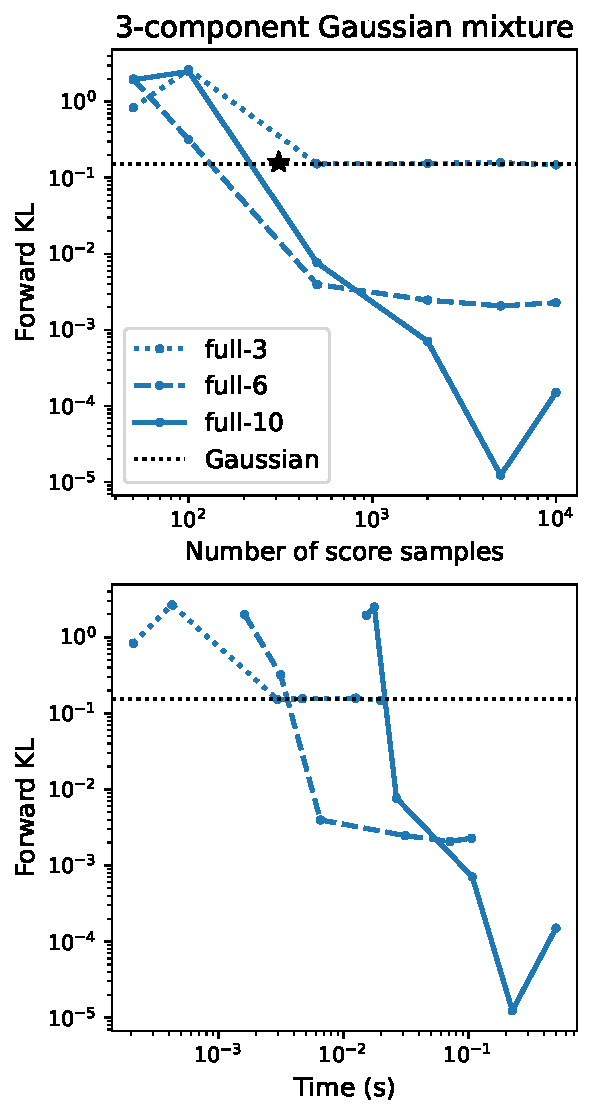
\includegraphics[scale=0.42]{figs/expts-2d/metrics-3gmm_full.pdf}
    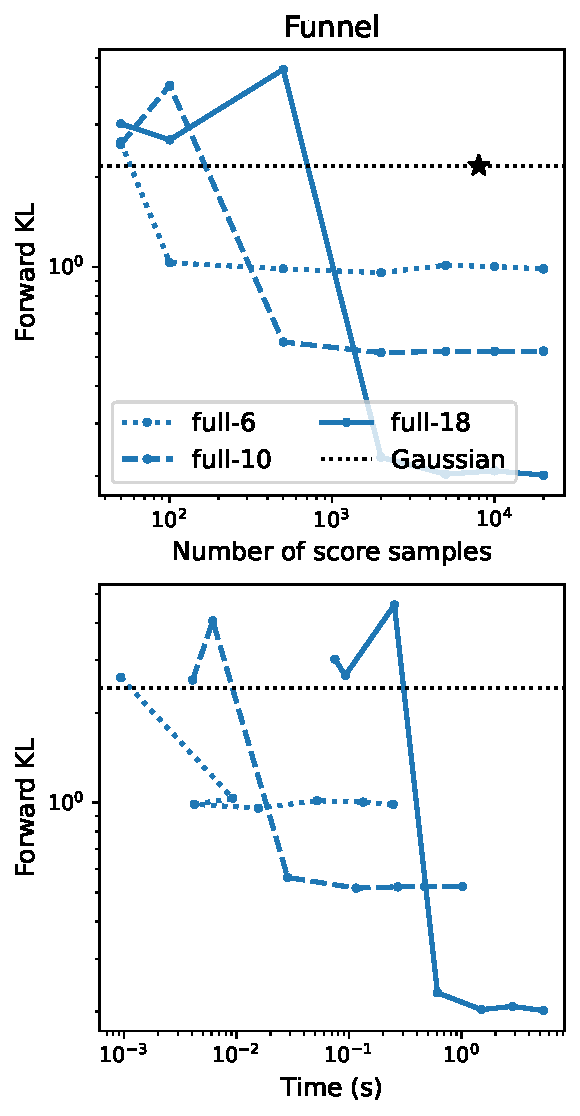
\includegraphics[scale=0.42]{figs/expts-2d/metrics-funnel_full.pdf}
    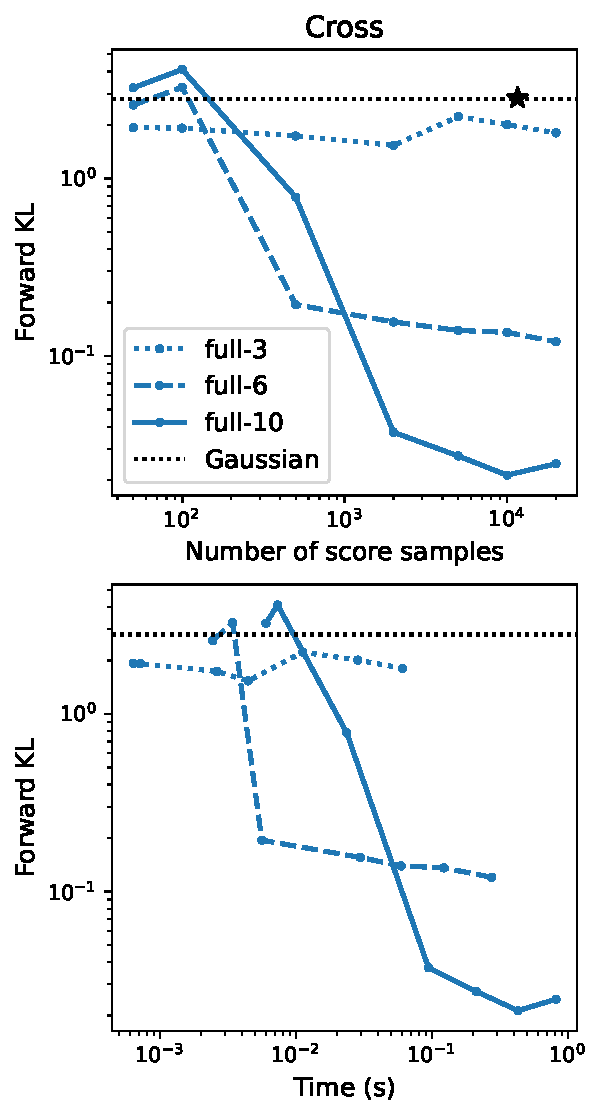
\includegraphics[scale=0.42]{figs/expts-2d/metrics-cross_full.pdf}
    \caption{We compare the number of score evaluations wallclock vs
FKL divergence for the target distributions in
\Cref{fig:2dtargets}: the Gaussian mixture (column 1),
the funnel (column 2), and
the cross (column 3) distributions.
The $K$ used for EigenVI is reported in each figure legend,
where $K=K_1 K_2$.
The black star denotes the number of gradient evaluations for the Gaussian method.
    }
\label{fig:2dtargets-metrics}
\end{figure}

We considered the following synthetic 2D targets:

\begin{itemize}

    \item \textbf{3-component Gaussian mixture:}
    \begin{align*}
    p(z) =
    0.4 \N(z \given [-1,1]^\top,\Sigma)
    +
    0.3 \N(z \given  [1.1,1.1]^\top,0.5I)
    +
    0.3 \N(z \given [-1,-1]^\top,0.5I),
\end{align*}
where we define
$\Sigma =
\begin{bmatrix}
    2 & 0.1 \\
    0.1 & 2 \\
\end{bmatrix}$.


\item \textbf{Funnel distribution with $\sigma^2=1.2$:}
\begin{align*}
    p(z) = \N(z_1 \given 0, \sigma^2) \N(z_2 \given 0, \exp(z_1/2)).
\end{align*}

\item \textbf{ Cross distribution:}
\begin{align*}
    p(z) =
    \tfrac{1}{4} \N(z \given [0,2]^\top,\Sigma_1)
    +
     \tfrac{1}{4} \N(z \given [-2,0]^\top,\Sigma_2)
    +
     \tfrac{1}{4} \N(z \given  [2,0]^\top,\Sigma_2)
    +
     \tfrac{1}{4} \N(z \given  [0,-2]^\top,\Sigma_1),
\end{align*}
where
$\Sigma_1 = \begin{bmatrix}
0.15^{0.9} & 0 \\ 0 & 1
\end{bmatrix}$
and
$\Sigma_2 = \begin{bmatrix}
    1 & 0 \\
0 & 0.15^{0.9}
\end{bmatrix}$.

\end{itemize}

These experiments were conducted without standardization with a Gaussian VI estimate.
The EigenVI proposal distribution $\pi$ used was a $\text{uniform}([-9,9])$ distribution.

In  \Cref{fig:5dtargetdensity}, we run EigenVI for increasing numbers of importance samples $B$
and report the resulting forward KL divergence.
The blue curves denote variational families with different $K_1=K_2=K$ values used,
i.e., 3, 6, and 10 (resulting in a total
number of basis functions of $3^2$, $6^2$, and $10^2$).
In the bottom row of the plot, we also show wall clock timings (computed without parallelization)
to show how the cost grows with the increase in the number of basis functions and importance samples.
The horizontal dotted line denotes the result from batch and match VI,
which fits a Gaussian via score matching; here a batch size of 16 was used
and a learning rate of $\lambda_t = \tfrac{BD}{t+1}$.

The black star denotes the number of score evaluations used by the Gaussian
VI method.


\subsection{Sinh-arcsinh targets}
\label{ssec-sinh}

The sinh-arcsinh normal distribution \citep{jones2009sinh,jones2019sinh}
has parameters $s \in \reals^D, \tau \in \reals_+^D, \Sigma \in \mathbb{S}_{++}$;
it is induced by transforming a
Gaussian $Z_0 \sim \N(0, \Sigma)$ to $Z = \mathcal{S}_{s,\tau}(Z_0)$,
where
\begin{align}
\mathcal{S}_{s,\tau}(z) :=
    [S_{s_1,\tau_1}(z_1), \ldots, S_{s_D,\tau_D}(z_D)]^\top,
    \quad
S_{s_d,\tau_d}(z_d) := \sinh\left(\tfrac{1}{\tau_d} \sinh^{-1}(z_d) + \tfrac{s_d}{\tau_d}\right).
\end{align}
Here $s_d$ controls the amount of skew in the $d$th dimension,
and $\tau_d$ controls the tail weight in that dimension.
When $s_d\!=\!{0}$ and $\tau_d\!=\!{1}$ in all dimensions $d$, the distribution is Gaussian. % the Gaussian distribution.



The sinh-arcsinh normal distribution has the following density:
\begin{align}
p(z; s, \tau, \Sigma)
    = [(2\pi)^D |\Sigma|]^{-\frac{1}{2}}
    \prod_{d=1}^D
    \left\{
        (1 + z_d^2)^{-\frac{1}{2}}
\tau_d \, C_{s_d, \tau_d}(z_d)
    \right\}
\exp\left(-\frac{1}{2} S_{s,\tau}(z)^\top \Sigma^{-1} S_{s,\tau}\right),
\end{align}
where we define the functions
\begin{align}
    C_{s_d,\tau_d}(z_d) := (1 + S_{s_d,\tau_d}^2(z))^{\frac{1}{2}},
\end{align}
and
\begin{align}
    \quad
    S_{s_d,\tau_d}(z_d) := \sinh(\tau_d \sinh^{-1}(z_d) - s_d),
    \quad
    S_{s,\tau}(z) =
    [S_{s_1,\tau_1}(z_1), \ldots, S_{s_D,\tau_D}(z_D)]^\top.
\end{align}

We constructed 3 targets in 2 dimensions and 3 targets in 5 dimensions,
each with varying amounts of non-Gaussianity.
The details of each target are below.
In all experiments, EigenVI was applied with standardization,
where a Gaussian was fit using batch and match VI with a batch size of 16
and a learning rate $\lambda_t = \tfrac{BD}{t+1}$.
%


For all experiments, we used a proposal distribution $\pi$
that was uniform on $[-5,5]^2$.

\begin{figure}[t]
    \centering
    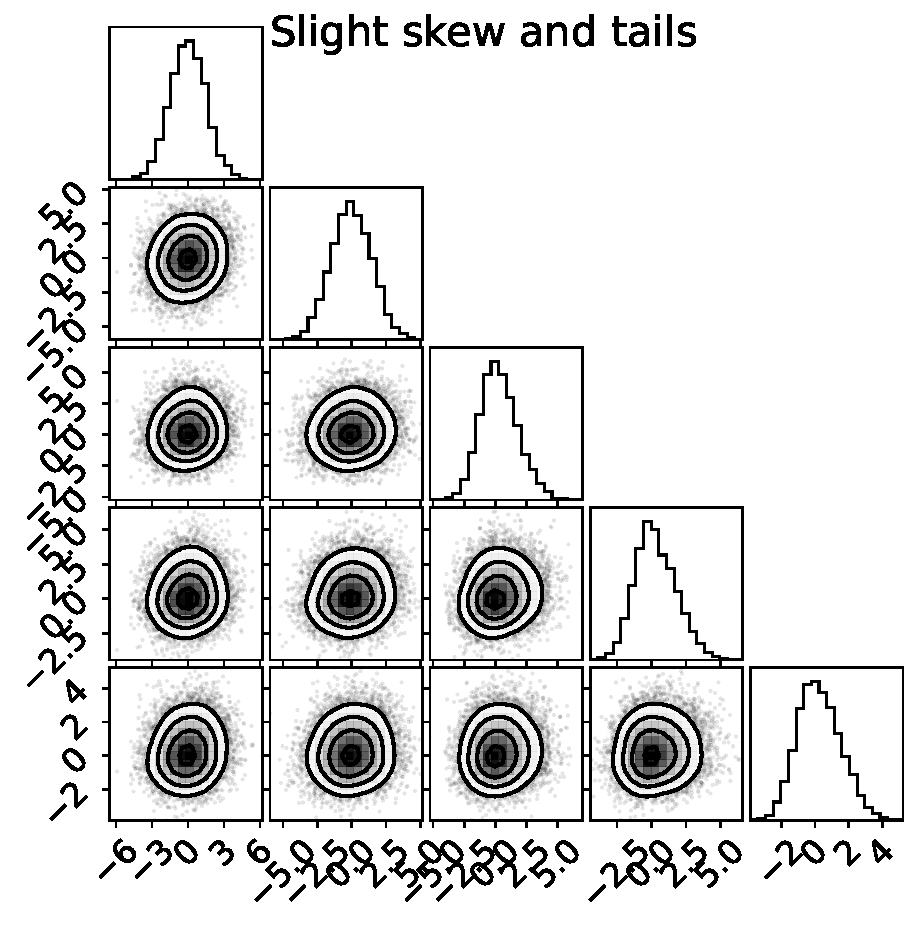
\includegraphics[scale=0.28]{figs/expts-2d/sinh_5D_target1v2.pdf}
    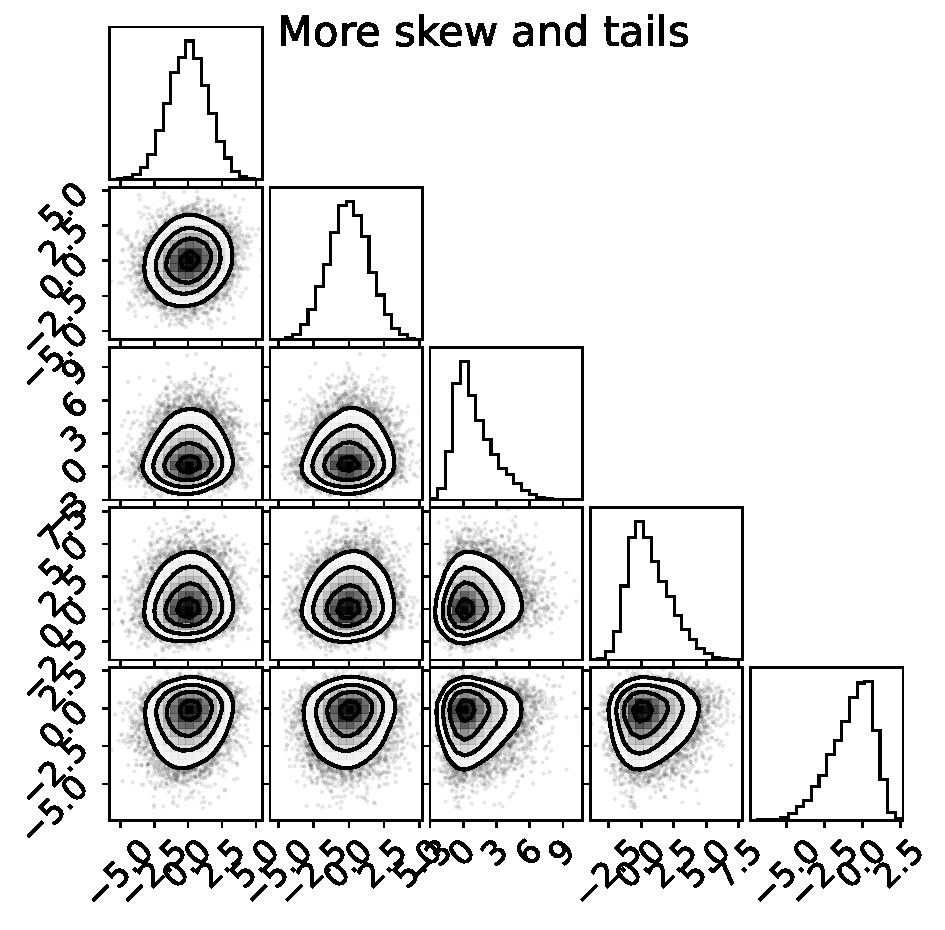
\includegraphics[scale=0.28]{figs/expts-2d/sinh_5D_target2v2.pdf}
    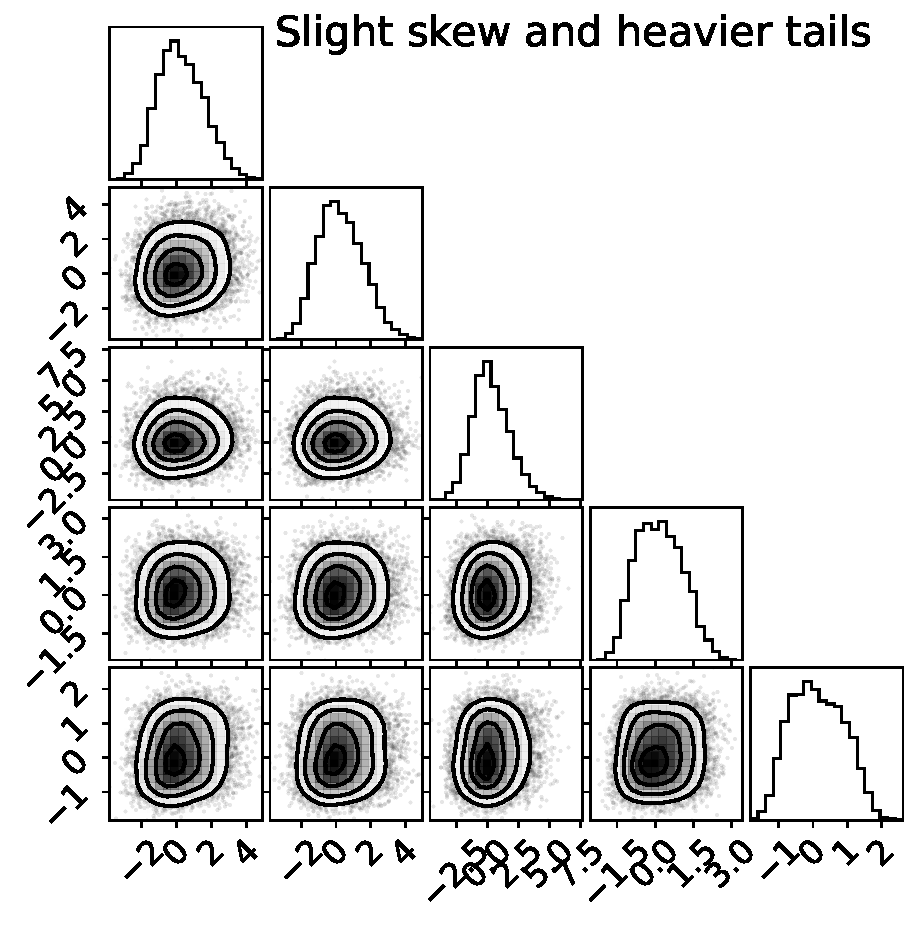
\includegraphics[scale=0.28]{figs/expts-2d/sinh_5D_target3v2.pdf}
    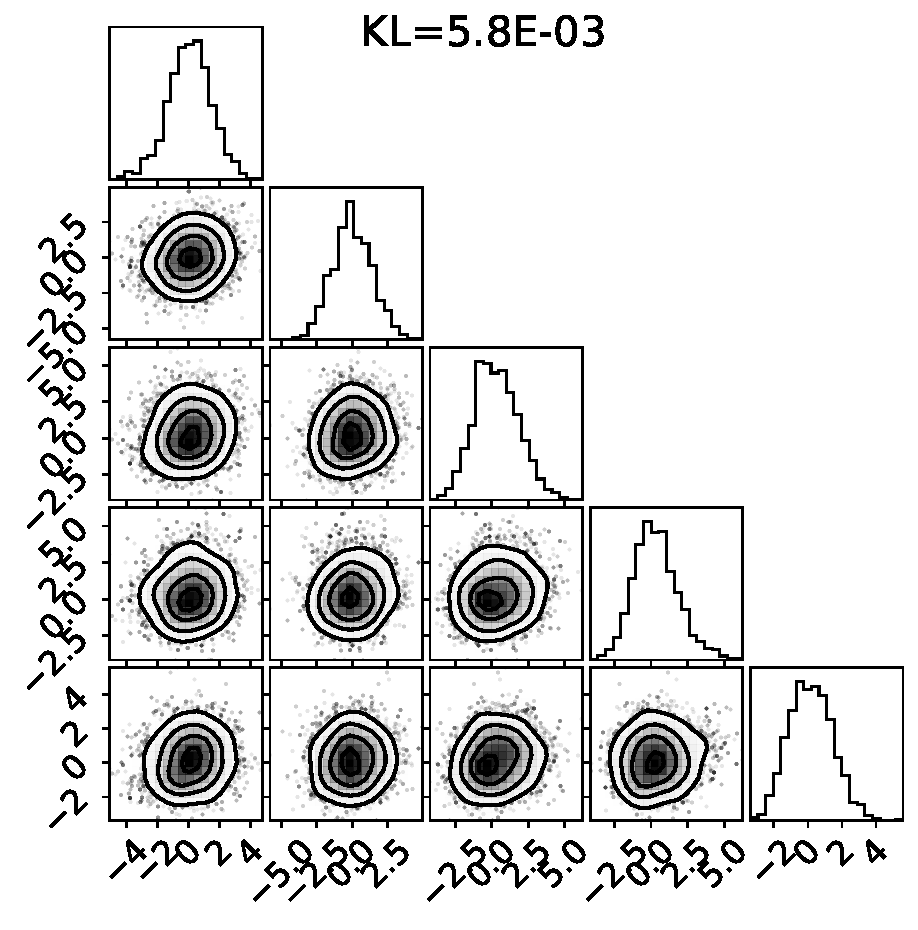
\includegraphics[scale=0.28]{figs/expts-2d/sinh_5D_target1-fit.pdf}
    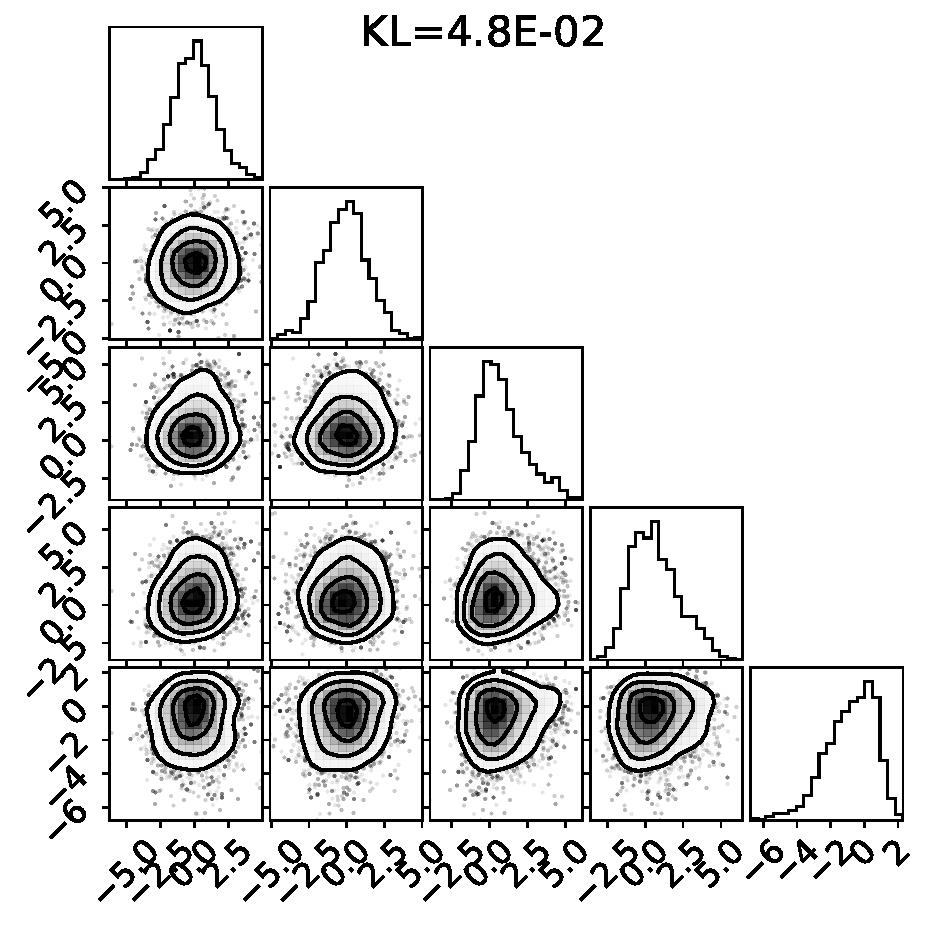
\includegraphics[scale=0.28]{figs/expts-2d/sinh_5D_target2-fit.pdf}
    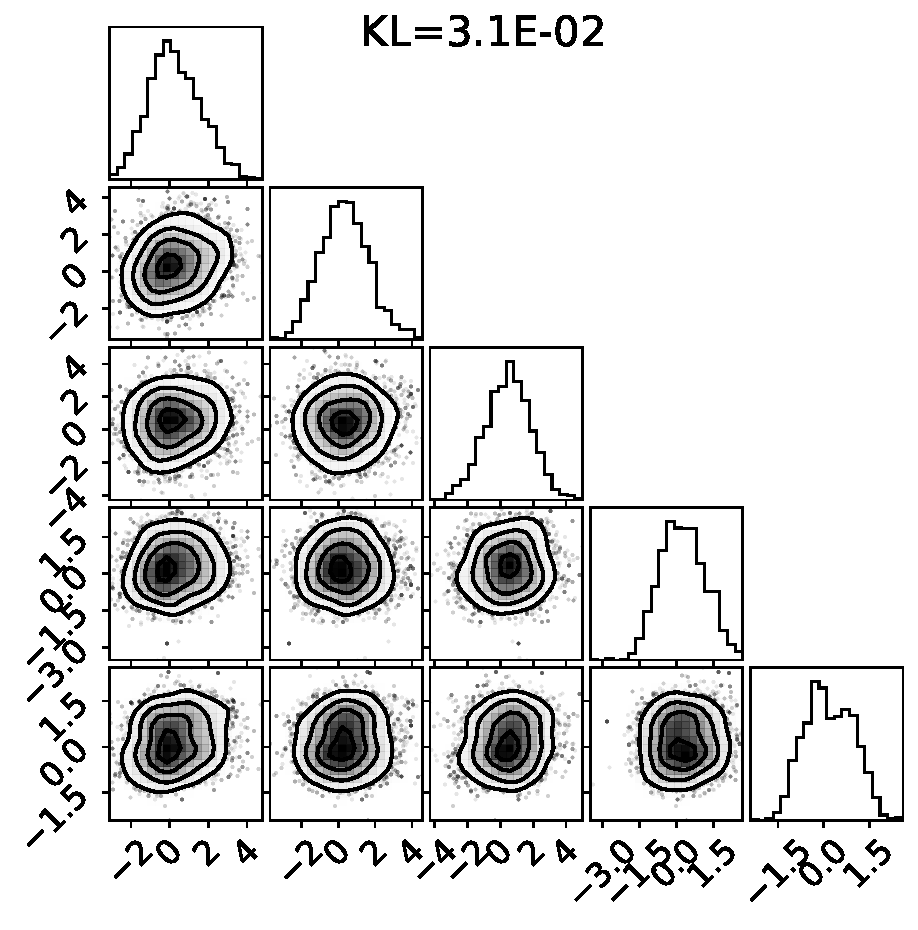
\includegraphics[scale=0.28]{figs/expts-2d/sinh_5D_target3-fit.pdf}
\caption{Targets (top) for the 5D sinh-arcsinh normal distribution example
and EigenVI fits (bottom) with the KL divergence in the figure title.}
\label{fig:5dtargetdensity}
\end{figure}

\paragraph{2D sinh-arcsinh normal experiment}
For $D=2$ (\Cref{subfig:sinh2D}), we consider the
\emph{slight skew and tails target} with parameters
$s=[0.2,0.2], \tau = [1.1,1.1]$,
the \emph{more skew and tails target} with
$s=[0.2,0.5], \tau = [1.1,1.1]$,
and \emph{the slight skew and heavier tails} with
$s=[0.2,0.2], \tau = [1.4,1.1]$.
Note that $s=[0,0], \tau=[1,1]$ recovers the multivariate Gaussian.
%
These three target are visualized in
\Cref{fig:sinh2dtargets}.

\paragraph{5D sinh-archsinh normal experiment}


We constructed three targets $P_1$ (slight skew and tails), $P_2$ (more skew and tails),
and $P_3$ (slight skew and heavier tails) each with
\begin{align}
    \Sigma =
\begin{bmatrix}
    2.2 & 0.3 & 0   & 0   & 0.3 \\
    0.3 & 2.2 & 0   & 0   & 0 \\
    0   & 0   & 2.2 & 0.3 & 0 \\
    0   & 0   & 0.3 & 2.2 & 0 \\
    0.3 & 0   & 0   & 0   & 2.2 \\
\end{bmatrix}.
\end{align}
The skew and tail weight parameters used were:
$s_1 = [0.,0.,0.2,0.2,0.2]; \tau_1 = [1., 1., 1., 1., 1.1]$,
$s_2 = [0.0,0.0,0.6,0.4,-0.5]; \tau_2 = [1., 1., 1., 1., 1.1]$,
and
$s_3 = [0.2,0.2,0.2,0.2,0.2]; \tau_3 = [1.1, 1.1, 1., 1.4, 1.6]$.
See \Cref{fig:5dtargetdensity} for a visualization of the marginals of each target distribution.
In the second row, we show examples of resulting EigenVI fit (visualized using samples from $q$)
from $B=20{,}000$ and $K=10$.


\subsection{Posteriordb experiments}
\label{ssec:pdb}

We consider 8 real data targets from \texttt{posteriordb}, a suite of benchmark
Bayesian models for real data problems.
In \Cref{table:posteriordb}, we summarize the models considered in the study.
These target distributions are non-Gaussian, typically with some skew or different tails.
To access the log target probability and their gradients, we used the
BridgeStan library \citep{roualdes2023bridgestan}, which by default transforms the target
to be supported on $\reals^D$.

For all experiments, we fixed the number of importance samples to be
$B=40{,}000$; to construct the EigenVI matrix $M$, the computations were parallelized
over the samples.
These experiments were repeated over 5 random seeds, and we report the mean and standard errors in
\Cref{fig:posteriordb}; for lower dimensions, there was little variation between runs.

The target distributions were standardized using a Gaussian fit from score matching
before applying EigenVI.
In most cases, the proposal distribution $\pi$ was chosen to be uniform over $[-6,6]^D$.
For the models \texttt{8-schools},
which has a longer tail, we used a multivariate Gaussian proposal with zero mean
and a scaled diagonal covariance $\sigma I$, with $\sigma = 3^2$.

\begin{table}
\caption{Summary of \texttt{posteriordb} models}
\label{table:posteriordb}
    \centering
    \small
\begin{tabular}{ccc}
    \toprule
    Name & Dimension & Model description \\
    \midrule
    \texttt{kidscore} & 3 & linear model with a Cauchy noise prior \\
   % \texttt{earn-height} & 3 & linear model with uniform prior \\
    \texttt{sesame} & 3 & linear model with uniform prior \\
    \texttt{gp\_regr} & 3 & Gaussian process regression with squared exponential kernel \\
    \texttt{garch11} & 4 & generalized autoregressive conditional heteroscedastic model \\
    \texttt{logearn} & 4 & log-log linear model with multiple predictors \\
    \texttt{arK-arK} & 7 & autoregressive model for time series \\
    \texttt{logmesquite} & 7 & multiple predictors log-log model  \\
    %\texttt{bball-hmm} & 8 & hidden Markov model with exponential distribution emissions \\
    \texttt{8-schools} & 10 & non-centered hierarchical model for 8-schools \\
    \bottomrule
\end{tabular}
\end{table}


\begin{figure}
    \centering
    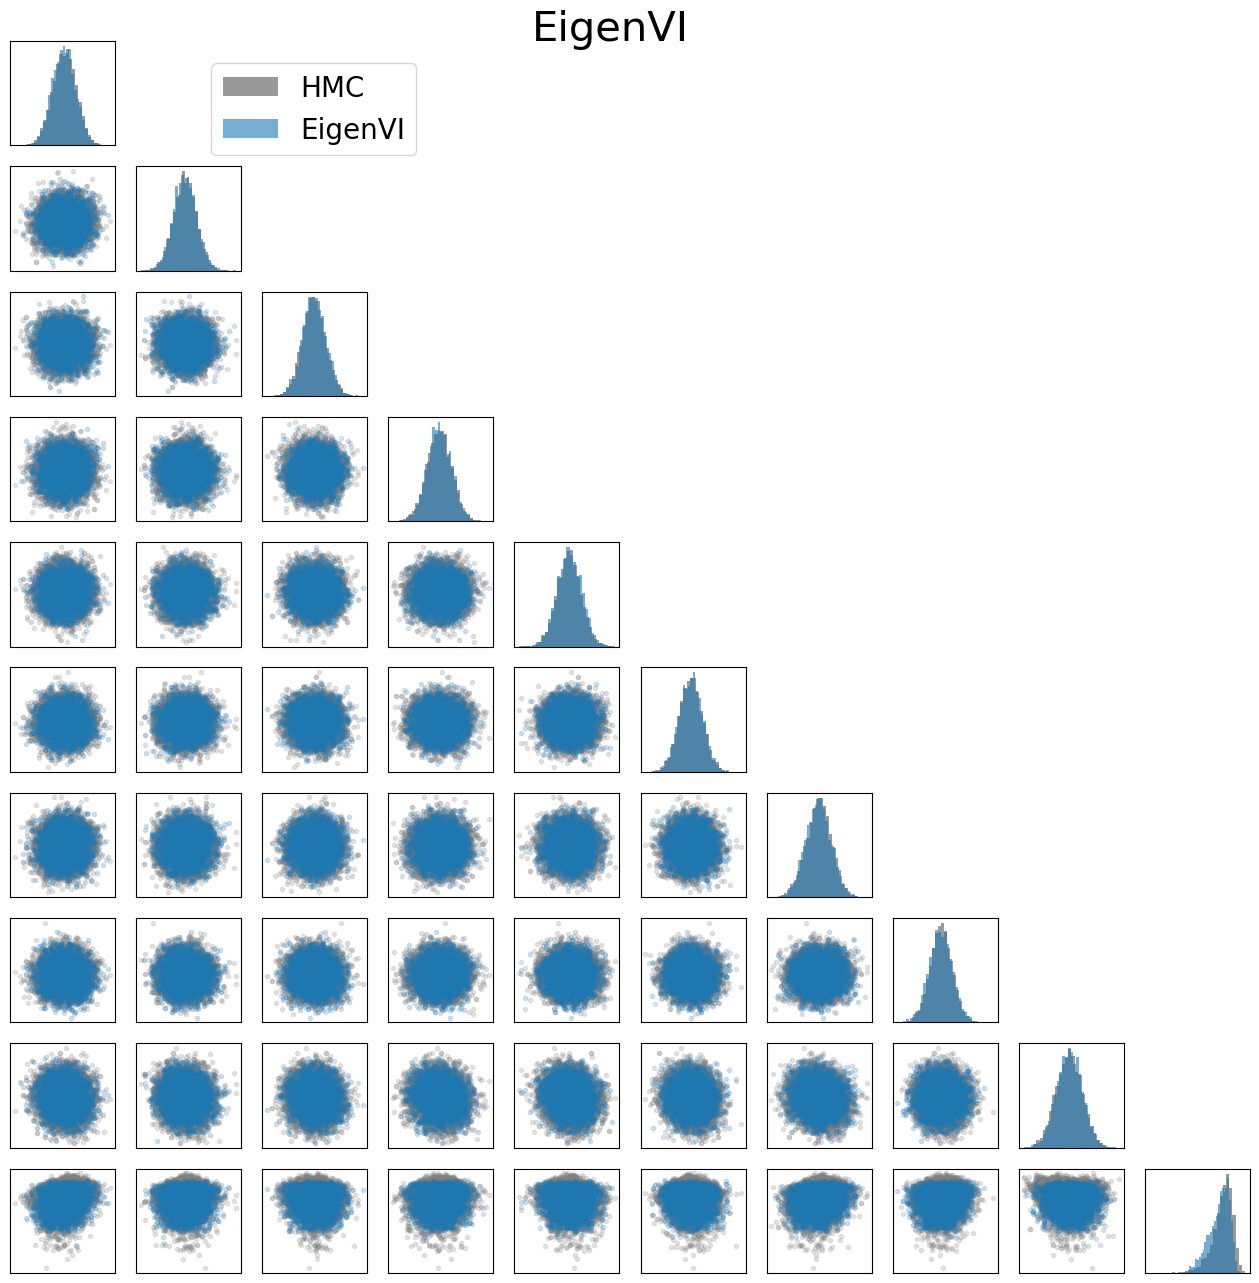
\includegraphics[scale=0.23]{figs/expts-pdb/PDB_85_corner_eigenvi.png}
    \\
    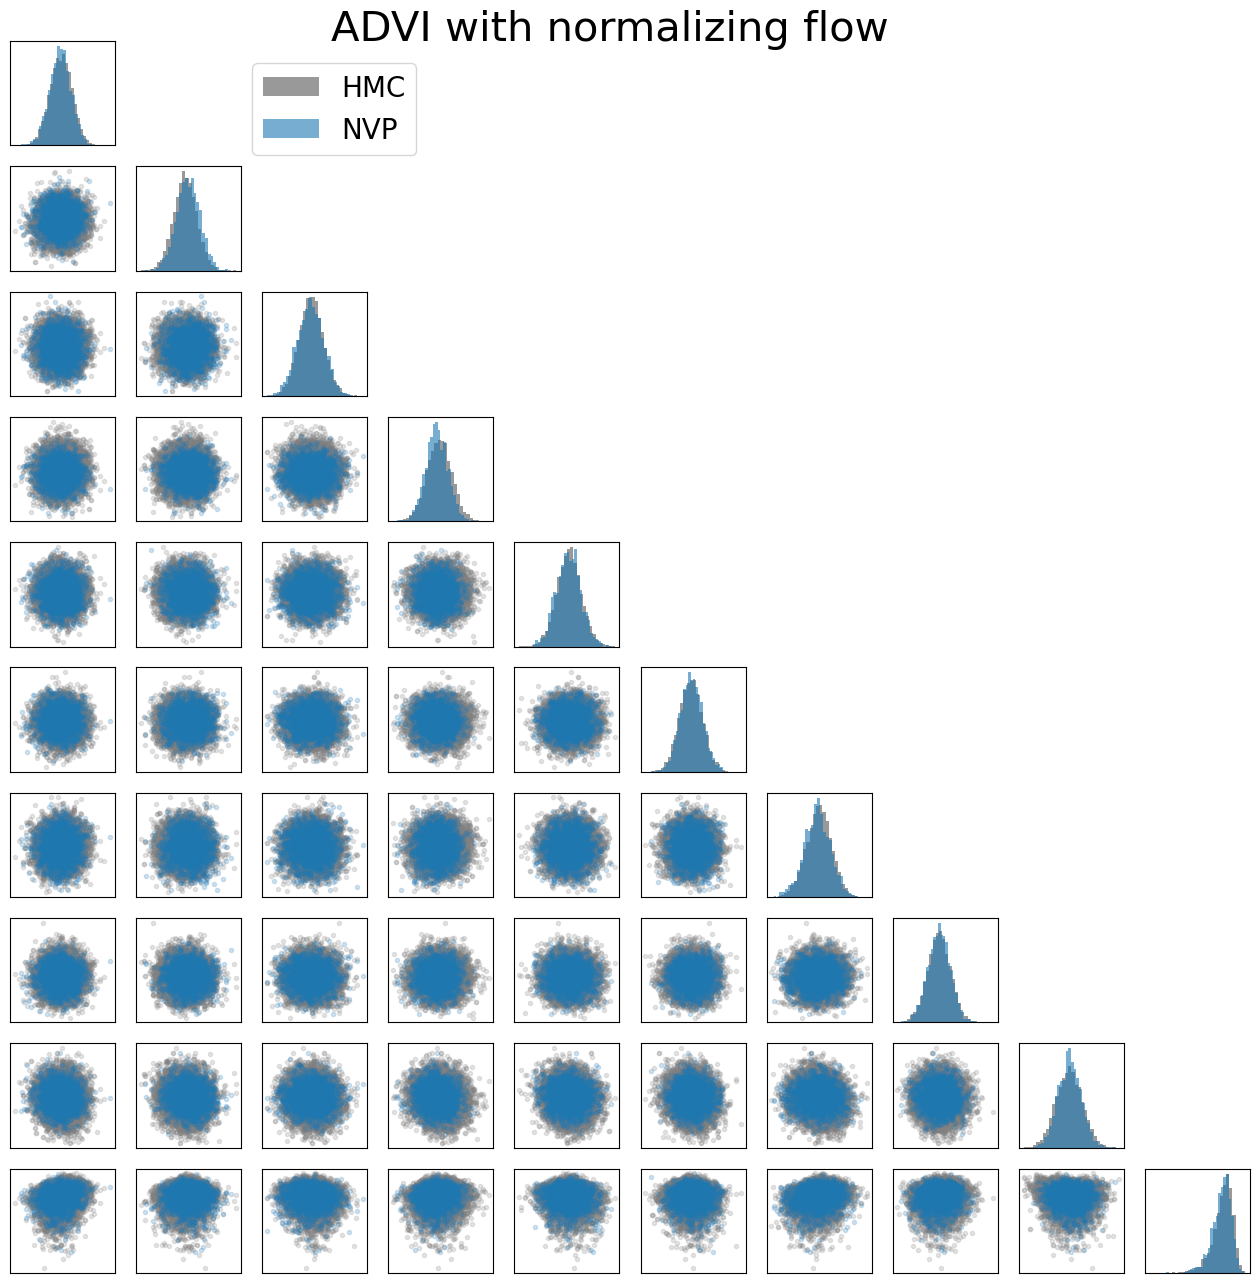
\includegraphics[scale=0.23]{figs/expts-pdb/PDB_85_corner_flows.png}
    \\
    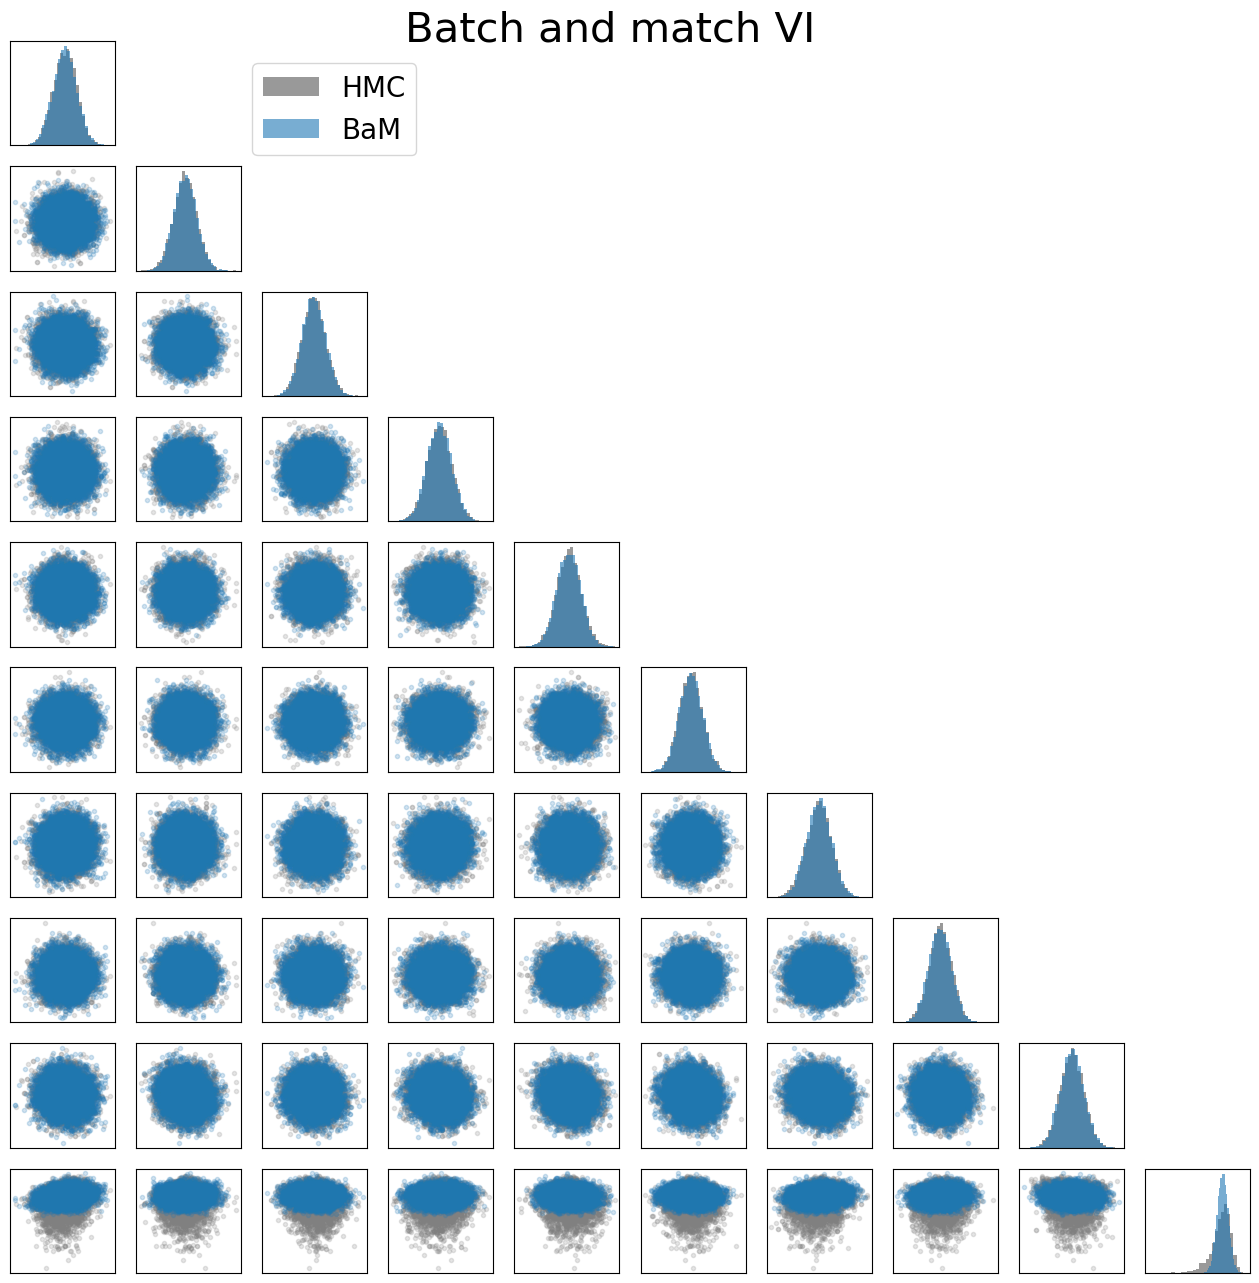
\includegraphics[scale=0.23]{figs/expts-pdb/PDB_85_corner_bam.png}
    \caption{Comparison of EigenVI, normalizing flow,
    and Gaussian score-based BBVI methods on
\texttt{8schools}.
    }
\label{fig:8schools:corner}
\end{figure}

\begin{figure}
    \centering
    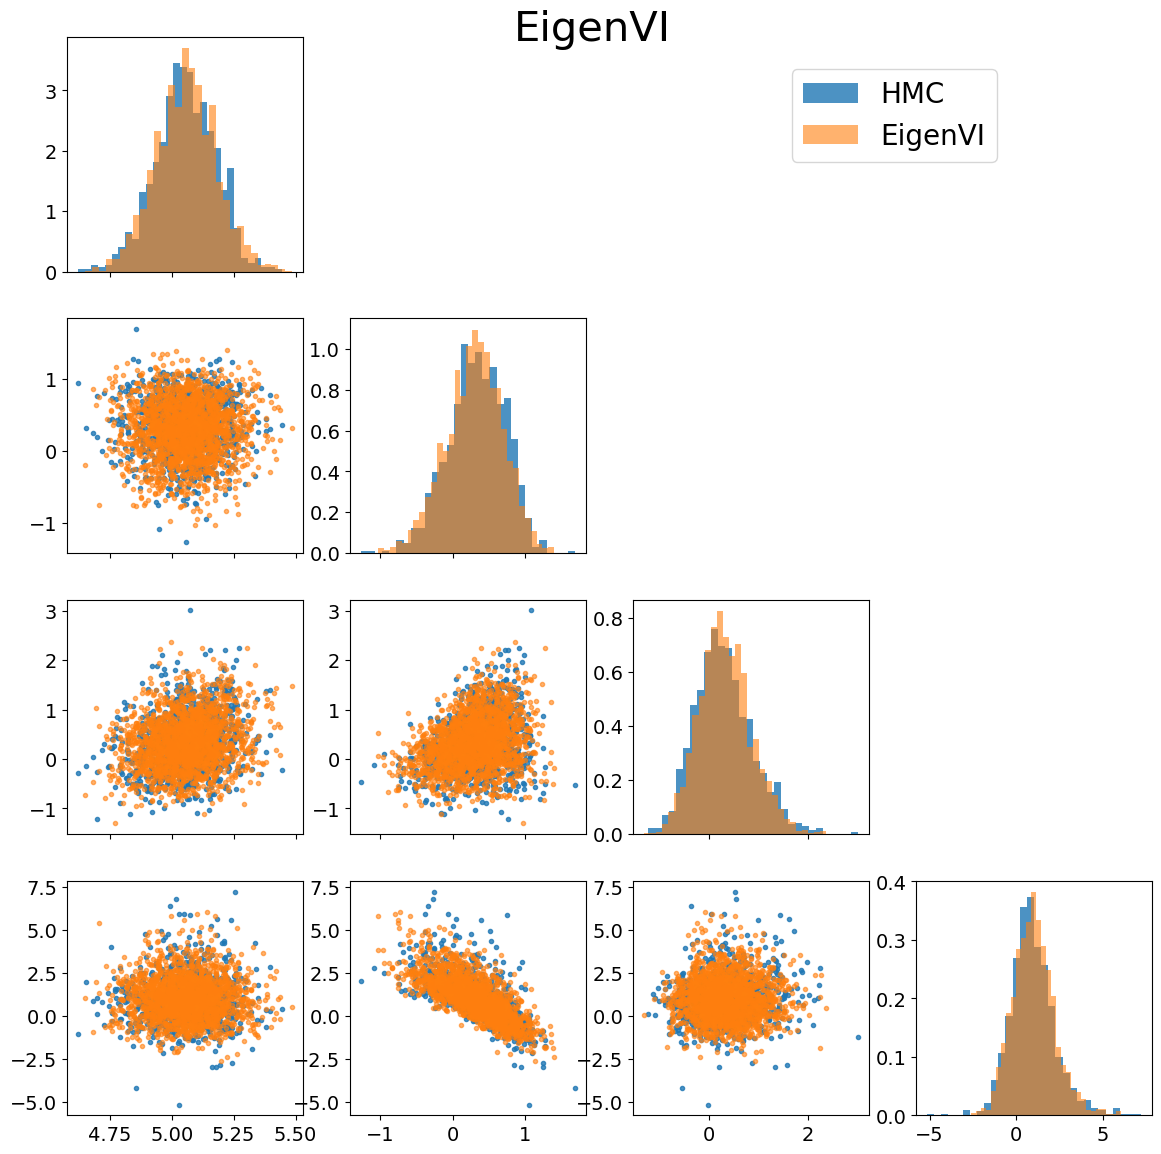
\includegraphics[scale=0.23]{figs/expts-pdb/PDB_99_samples_eigenvi.png}
    \\
    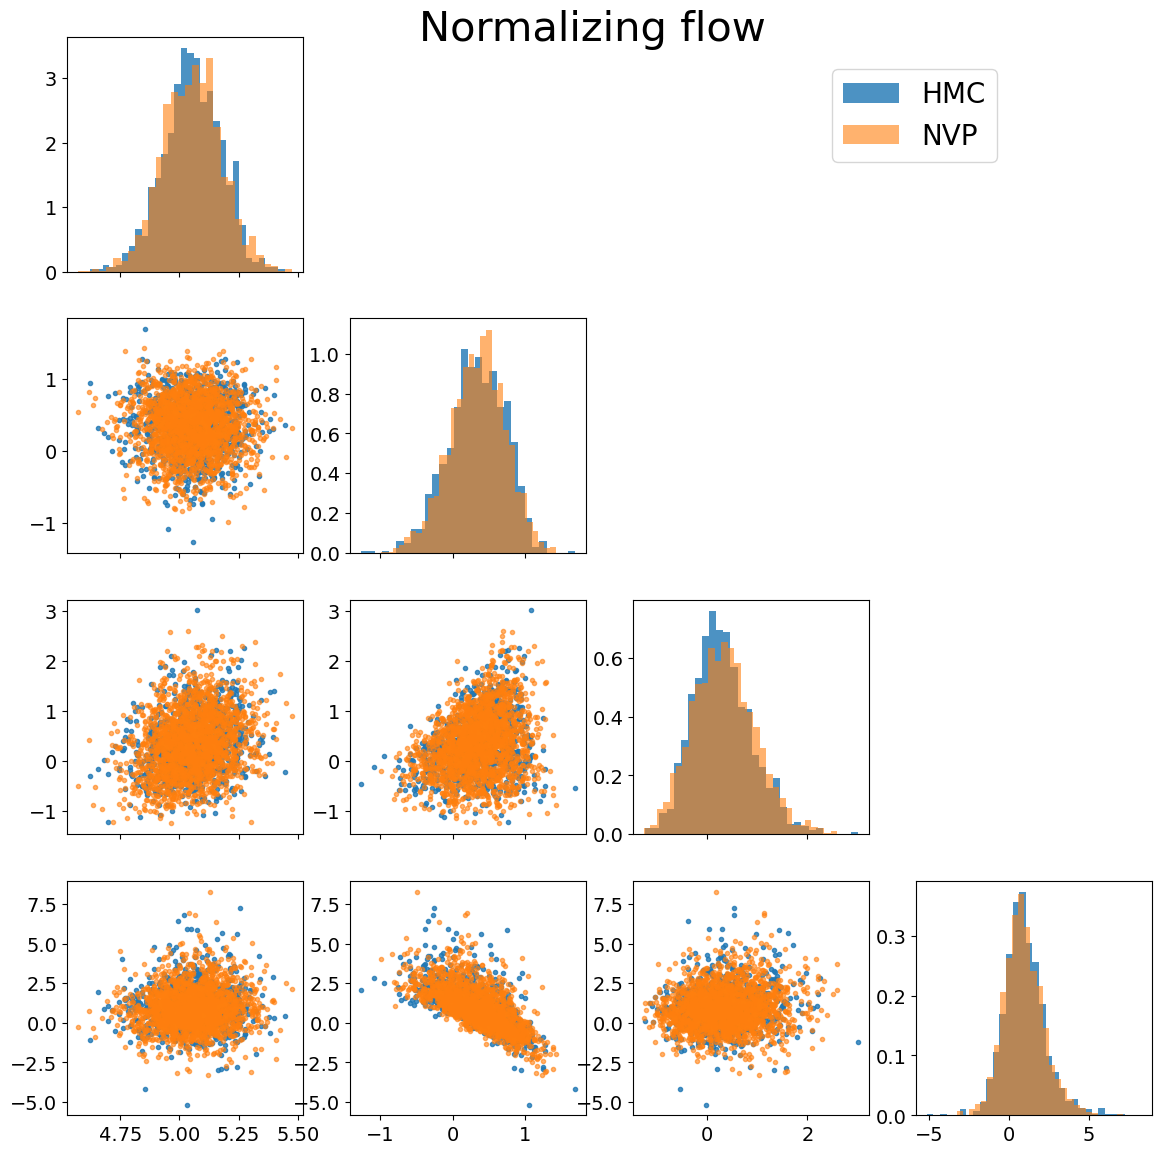
\includegraphics[scale=0.23]{figs/expts-pdb/PDB_99_samples_flow.png}
    \\
    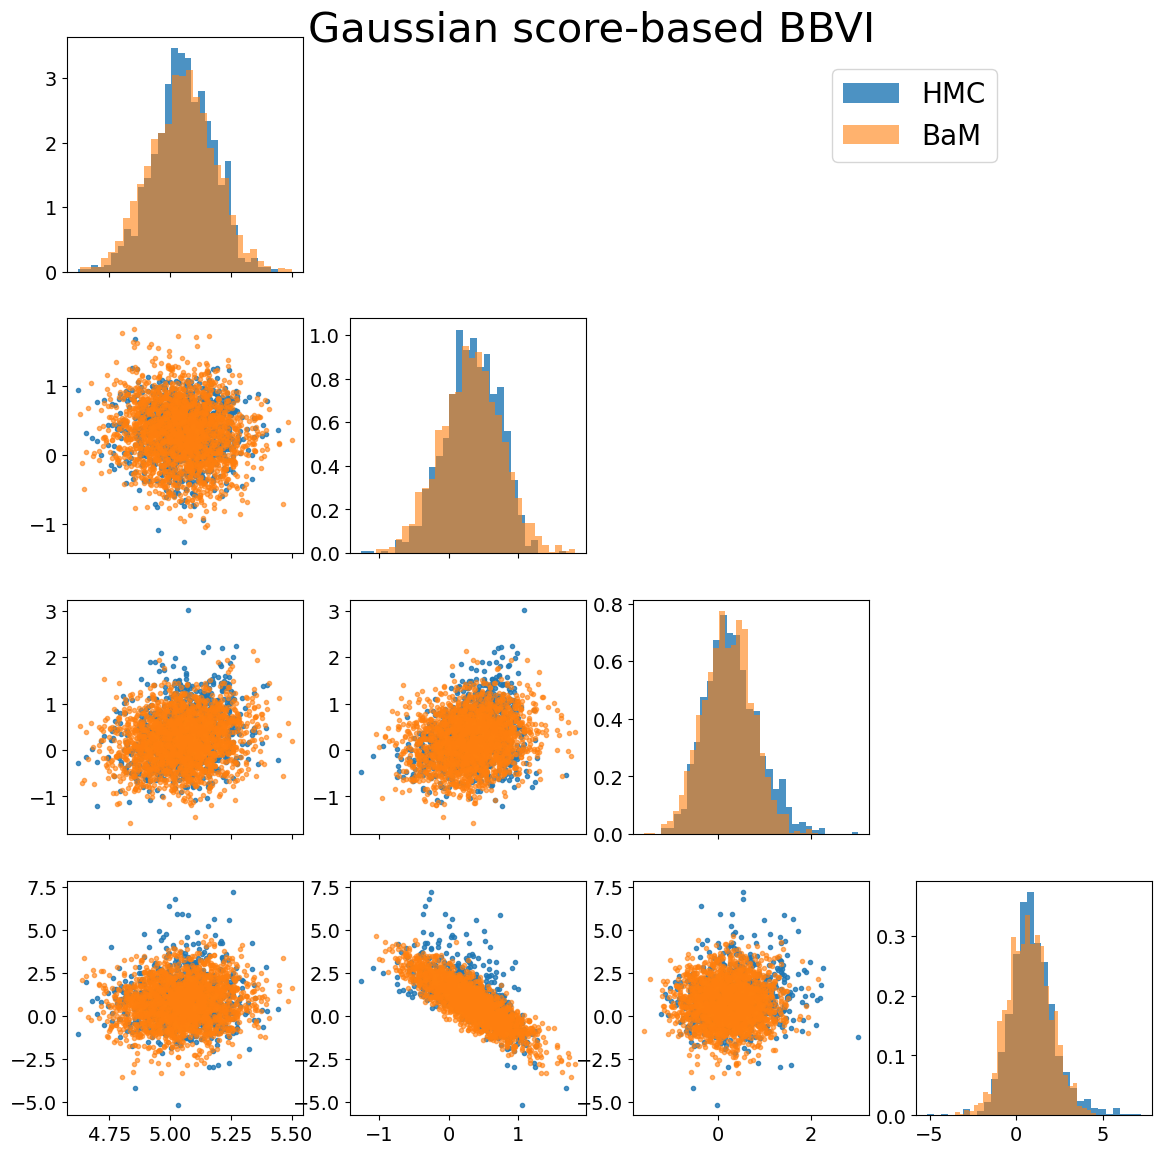
\includegraphics[scale=0.23]{figs/expts-pdb/PDB_99_samples_bam.png}
    \caption{Comparison of EigenVI, normalizing flow,
    and Gaussian score-based BBVI methods on
\texttt{garch11}.
Note that the Gaussian approximation over/underestimates the tails,
while the more expressive families fit the tails better.
    }
\label{fig:garch11:corner}
\end{figure}


For the Gaussian score matching (GSM) method \citep{modi2023},
we chose a batch size of 16 for all experiments. We generally found the
results were not too sensitive in comparison to other batch sizes of 4,8, and 32.
For the batch and match (BaM) method \citep{cai2024}, we chose a batch size of 16.
The learning rate was fixed at
$\lambda_t = \tfrac{BD}{t+1}$, which was a recommended schedule for non-Gaussian targets.

For all ELBO optimization methods (full covariance Gaussian family and normalizing flow family),
we used Adam to optimize the ELBO.
We performed a grid search over the learning rate
$0.01, 0.02, 0.05, 0.1$ and batch size $B=4,8,16,32$.
For the normalizing flow model,
we used a real NVP \citep{dinh2016density}
with 8 layers and 32 neurons.
We found empirically that the computational of the scores was unreliable~\cite{kohler2021smooth,
Zeghal2022npe};
hence we do not show their Fisher divergence in \Cref{fig:posteriordb}.


In \Cref{fig:8schools:corner}
and
\Cref{fig:garch11:corner},
we show the corner plots that compare an EigenVI fit, a normalizing flow fit, and a Gaussian fit
(BaM).
In each plot, we plot the samples from the variational distribution against
samples from Hamiltonian Monte Carlo.
We observe that the two more expressive families EigenVI and the normalizing flow
are able to model the tails of the distribution better than the Gaussian fit.

%\end{document}

